\chapter{Analysis}
\label{chap:analysis}

The debugging activity collected 6890 snapshots over 119 projects. The temperature activity collected 2296 snapshots over 35 projects. In total, 9186 snapshots were analyzed. From these data, features were extracted that represented the type of code change that occurred in a snapshot. After some analysis of these change-type features, a new analytical method was constructed to provide teachers with useful information towards identifying flailing, off-task, or disengaged behavior. The new method, called \emph{solution particle analysis,} did not depend on the change-type features, instead using purpose-specific new feature extractor. This technique is described below in Section \ref{sec:particle-analysis}.

The particle analysis method allowed for the development of a visual display tool that allowed immediate insight into the state of a classroom in the recorded data, in such a way that would aid a teacher in coordinate their resources. 

The process of generating the extracted features, which served as the raw data for all analysis techniques, is discussed below in Section \ref{sec:data-processing}.


\section{Data Processing Pipeline}
\label{sec:data-processing}
% Data Pipeline:
% filter to relevant projects in database ->
% processProject:
%	load change contents from git
%		fix trailing xml corruption
%		checks for empty blocks, only includes if not-empty
%		generate IDmaps and parentmaps
%	extract changes
%		check for:
%			added/Deleted blocks
%			movedblocks
%			contextMove
%			changedblocks
%			fieldchanges
% 	reduceFieldChanges
%	generateChangeIntervals

Data was imported from the git database into the analysis environment using a process shown in Figure \ref{fig:data-import-process}. The key step of this process was ``Extract change features,'' where the tests for the types of changes in that snapshot were executed. Feature extraction is described in detail below in Section \ref{sec:feature-extraction}.

\begin{figure}
  \centering
      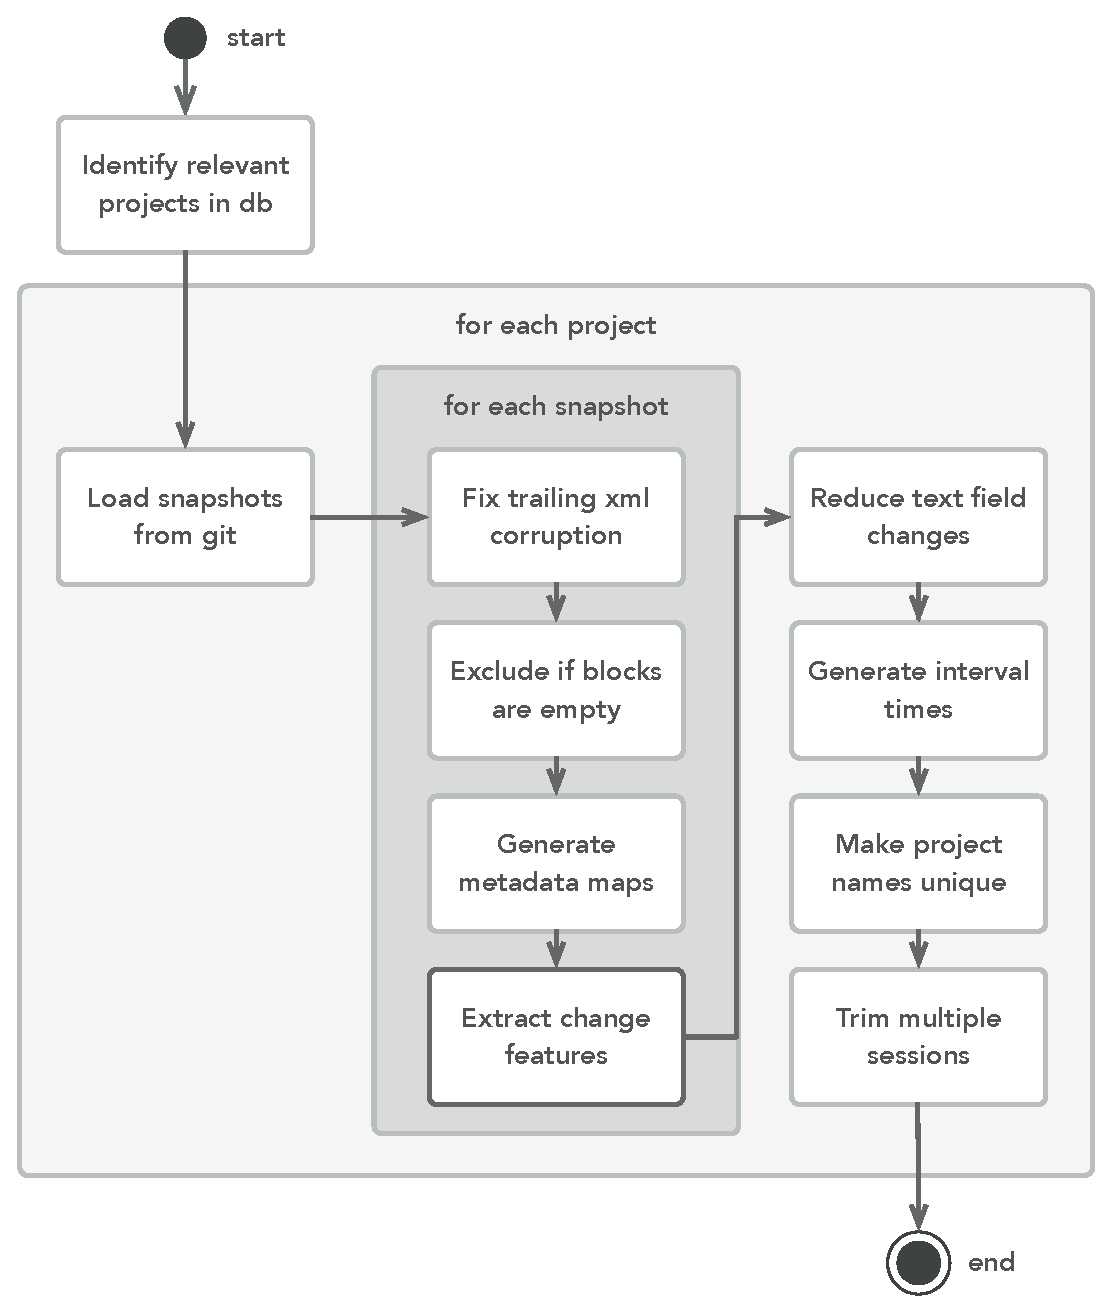
\includegraphics[width=\textwidth]{diagrams/data-import-process}
  \caption[The Data Importing Process]{The data importing process. The entire database was scanned for projects that contain an identifiable element, which were then loaded directly from git. Each change from git was processed for error mitigation and necessary metadata generation, then the features were extracted. After feature extraction, character-wise text field changes were reduced, and then the interval times between snapshots were generated.}
  \label{fig:data-import-process}
\end{figure}

The import pipeline had many tasks to accomplish, starting with identifying the projects that were relevant for analysis. The App Inventor instance that was used for this study was also used for the entirety of the summer camp curricula, so there were many projects captured in the snapshot database that were not part of the activities specific to this study. This was an intentional part of the protocol to make transition easier for the camp students by only having one App Inventor instance with which to interface. The in-class activities were better isolated, so researchers were able to prepare the room in advance to steer the students transparently towards the specialized instance. 

The activities that were part of this study needed to be found in the database. Students had the ability to rename projects at any point, so it was possible (albeit unlikely) that a relevant project could be renamed. Therefore the protocol included a unique element in the projects, a ``magic string'' in a hard-to-find property of the project. The debugging activity and temperature activity each had a unique identifier string, and these strings were included in the starter code that all students were given. These unique elements were then detectable by scanning the files in the git database prior to import. There were instances of students changing the names of the projects, which demonstrated the need of the unique identifier. 

Once a list of projects were identified using their unique elements, those projects were loaded from git into the analysis environment. The git interface opened each project's repository, extracted a list of all commits, and then checked out each commit in turn, capturing the contents of the files for each commit. A commit represented a single snapshot, and the terms ``snapshot'' and ``change'' were used interchangeably to describe the contents of the commit after this stage. 

Each snapshot was checked for corruption at time of import. Following that, two metadata maps were generated for each snapshot: a map of block ID numbers, and a map of block parents. These maps allowed the feature extractor to easily access a block by its ID number (which would require a full tree traversal without), and easily look up the parent of any given block. With the maps generated, the feature extractor would then be able to run. 

After feature extraction, the text field events were reduced (described below), and finally, with the snapshot set complete, interval times between snapshots were generated.

Most stages of the import process were additive and non-destructive, so at the conclusion of import each project and snapshot had all of the data available at all previous steps. For instance, the raw block contents were not lost during feature extraction; the list of features were added to the data structure alongside it. 

The following sections delve further into certain components of the import pipeline, and are presented in pipeline order: corruption mitigation, feature extraction, and text field reduction.


\subsection{Corruption Detection and Mitigation}
Some forms of corruption were found in the snapshot data, all concerning the blocks representation. There were four corruption modes, which are explained below, with their respective mitigation strategies.

The first corruption mode was malformed XML files which contained text beyond the closing XML tag. This, of course, crashed the XML parser. Within the debugging activities, only seven snapshots had this malformation, which were corrected by trimming the excess text. It was noteworthy in those cases that the junk excess text was a repetition of the last characters of the file, lends to a hypothesis of the source of the corruption, discussed below.

The second form was rare, where a snapshot had no contents for the blocks file. In the entire collection of debugging activity snapshots ($n = 6890$), only three snapshots had empty blocks. These snapshots were detected during import and were not included in the research data. The overall history of the projects containing these empty shapshots were unaffected. 

Both of these corruptions were indicative of a bug in the extraction of the block data from blockly in the browser. It was possible that the snapshot mechanism was able to capture the XML file while it was in an inconsistent state, such as mid-write. This bug may be within the Blockly framework itself, and further investigation is recommended before attempting larger-scale deployment of this method.

The two above corruptions were easily mitigated. A third mode of corruption, however, resulted in properly formed XML, but potentially erroneous data. This mode was characterized by multiple changes happening in a single snapshot, which should have been extremely rare, as each snapshot was triggered by an atomic action in the editor. In reality, there was a small amount of caching in the capture mechanism, as discussed in Section \ref{sec:mod-ai}, which may have contributed to this corruption. There was no inherent problem with multiple changes in a single snapshot, if they all occured within the capture window of that snapshot. In these erroneous cases, one or more actions appeared to be inconsistently represented over time, which caused git and the subsequent analysis tools to do, un-do, and re-do the same action in very small spans of time, artificially inflating the representation of those events. 

One project was particularly egregious, and showed this corruption in 71 of its 245 commits, rendering nearly a third of its data unreliable. That project was removed, which left only 50 such potential errors in the remainder of the database, many of which were mitigated by text field accumulator, described in Section \ref{sec:text-acc}. 

A data consistency bug was found where a project was opened over more than one session. In App Inventor, if a project was opened in a second, disjoint session, such as the following day, the block ID numbers change, causing the feature extractors to falsely over-report blocks being deleted and added, when really the same blocks have been re-numbered. The strategy employed was to ignore snapshots that occurred at a timestamp beyond the maximum time of the activity.

The total percentage of potentially erroneous snapshots in the debugging activity dataset was 0.84\%. These are summarized in Table \ref{tab:data-corruption}.

% % Debug:		empty blocks - 3 (now, many were hand-fixed, notes may indicate more)
% %				junk past tag - 7 (now, many were hand-fixed, notes may indicate more)
% %			6890 snapshots total
% % Temperature:	empty blocks - 1 
% %				junk past tag - 4 
% %			2296 snapshots total
	
\begin{table}
\begin{centering}
	\begin{tabular}{l r l p{5.4cm}}
	Corruption Mode 		& \multicolumn{2}{l}{Instance Count} 		& Mitigation Strategy 			\\ \hline
	Empty block file 						&  3 &(0.04\%) 				& snapshot deleted 						\\
	Junk beyond \mintinline{xml}|</xml>| 	&  7 &(0.1\%) 				& junk trimmed, snapshot kept 			\\
	Multiple changes 						& 50 &(0.7\%) 				& accepted as insignificant 			\\
	Multi-session 							&  3 &(0.04\%) 				& data past 40 minutes ignored
	\end{tabular}
	\caption[Data corruption modes]{Data corruption modes, their prevalence, and mitigation strategy.}
	\label{tab:data-corruption}
\end{centering}
\end{table}


\subsection{Feature Extractor}
\label{sec:feature-extraction}

\begin{table}
\begin{labeling}{Blocks Moved in Context}

	\item [Blocks Added] Block(s) were added to the workspace. Nearly always a single block.
	\item [Blocks Deleted] Block(s) were removed from the workspace.
	\item [Blocks Moved in Space] Block(s) moved position on the workspace, but did not necessarily change programmatic meaning.
	\item [Blocks Moved in Context] Block(s) changed programmatic position, indicating a new parent block and a different place in the app's control flow.
	\item [Fields Changed] A block's text field changed. Could be a text literal, a variable or procedure name, or a number literal.
	\item [Properties Modified] One or more properties of a block has changed, which could indicate use of the mutator to change a block's semantics (such as changing the number of addends in an addition block). Intended as a catch-all if the other tests missed something, and was rarely found in the data.
	
\end{labeling}
\caption[Features extracted from snapshots]{Features extracted from snapshot data.}
\label{tab:features-extracted}
\end{table}

The features extracted by this module were listed and described above in Figure \ref{tab:features-extracted}. This section outlines the specific definitions that constitute the feature tests. All of these tests operated on snapshots of the same project that were adjacent in time. They detected differences between the two, often utilizing the metadata maps described above in Section \ref{sec:data-processing}. Source code for these algorithms are presented in Appendix \ref{src:feature-extraction-tests}.

The test for \emph{Blocks Added} and \emph{Blocks Deleted} were the same routine, which assembled a list of blocks by their ID numbers for both snapshots and compared differences between those lists using set arithmetic. 

The test for \emph{Blocks Moved in Space} assembled a list of blocks that were present in both snapshots, and iterated that list looking for blocks who were both top-level and whose coordinates changed. There was an important distinction made here- blocks that were nested within other blocks were not top-level and therefore did not trigger the \emph{Blocks Moved in Space} flag when they moved as a consequence of their parent moving. Only blocks whose parent is the workspace itself may return positive from this test, and then, only if they actually moved on the workspace.

\emph{Blocks Moved in Context} was the opposite of the above test, where it detected if a block moved in computational context, indicated by a changed parent. Similarly, this test assembled a list of blocks common to both snapshots, and iterated across that list. The iteration checked if the parent for the block was the same in both snapshots, and returned true if they were not. 

To detect \emph{Fields Changed}, common blocks were listed and then filtered for field properties. Those fields were searched for cases where the value of the fields differed between the two snapshots.

The final test, \emph{Properties Modified} caught any other modifications to a block. This test was more complex. Like those above, it assembled a list of blocks present in both snapshots. It then ran an exhaustive element-wise equality check on each block, comparing the version in each snapshot. If the equality check returned true, that block did not change in any way. If the equality check was false, then lists of all children for both blocks were assembled, which included properties, data fields, mutator instructions, and other Blockly metadata. This step excluded text fields, as they were covered in a previous test. If the lengths of the lists of children were unequal, then the routine returned true, as these particular blocks definitely changed between the two snapshots. If they have the same number of children, then each pair of children were iterated, and the element-wise equal was applied to each of them, effectively running a first-level recursive equality test. If that test did not find any differences, then the routine returned false. That final false return is a condition that should be impossible, but was included defensively, as there may have been edge cases possible in Blockly that were not common in known to the researchers at the time of this design.


\subsection{Text Field Change Accumulator}
\label{sec:text-acc}
In the course of working on their activities, students often manipulated fields of text, including text literals, variable names, procedure names, and parameter names. Examples of blocks utilizing open text fields are shown in Figure \ref{fig:text-fields}. Whenever a text field was modified, the change event was triggered for every character. This was a degree of granularity too fine for meaningful analysis, as character modification events are considered too primitive to be of use \citep{omori2008change}. The snapshot system at runtime could not discern the beginning and end of field editing events, so the change event feature \emph{Fields Changed} from Table \ref{tab:features-extracted} was grossly over-represented. 

To combat this over-representation, sequences of character-wise change events needed to reduced to their final state, which then represented a single change at the same degree of abstraction as the surrounding block manipulations. This reduction was accomplished with an accumulator algorithm, which scanned a project's change history and identified uninterrupted sequences of field modifications to the same field. The algorithm deleted all but the final \emph{Fields Changed} events, leaving only the final state of the modification for further processing. This algorithm had a 10-second timeout, so sequential edits to the same field would be considered different events if there were more than 10 seconds between them. Changes to different field blocks were also considered a new event. This algorithm is shown and further explained in Appendix \ref{src:reduceFieldChanges}.

\begin{figure}
  \centering
      \includegraphics[width=\textwidth]{images/ch4-text-fields}
  \caption[Examples of Text Fields in App Inventor]{Examples of some text fields in App Inventor. All of the fields, represented by the text in shaded bubbles, could be edited arbitrarily by the student.}
  \label{fig:text-fields}
\end{figure}



\section{The Particle Analysis Method}
\label{sec:particle-analysis}

The purpose of this study was to develop a tool, informed by students' fine-grained programming activities, that can aid a teacher in deciding how to apply their resources during a lab session in real time. A significant insight was reached during analysis of the above change-type features, that such a tool could be constrained to standardized, ``on-rails'' programming assignments. These closed-ended assignments constitute the bulk of many curricula in use, such as those described by  \citet{gray2012teaching}, \citet{martin2015dual}, and \citet{morelli2015analyzing}, and are particularly common at the beginning of curricula, when students are still learning the basics. This situation would be the ideal use case for an orchestration aid. 

With this insight, and the constraint it brought, design began for both a visual tool to help a teacher orchestrate, and an analysis method to power it. The resulting method was \emph{particle analysis,} which borrowed its name from the behavior of atoms and molecules. With this method, a solution to an activity can be regarded as a complex molecule, which was built up out of smaller molecules, which were themselves composed of atoms. In this analogy, every individual block was an atom, and were combined on the workspace to make expressions, representing molecules. A solution to an activity was one or more of these molecules, which could have any number of atoms within it. The analogy could be further extended, admittedly weakly, to correspond the solution to an activity with the chemical definition of ``solution,'' a homogeneous mixture composed of two or more substances. 

When you get to the close-enough text analyzer, it calculates Levenshtein edit distance, using an algorithm proposed by \citet{hyyro2001explaining}.


\section{The Classroom Console}
\label{sec:classroom-console}

